\chapter{INTRODUCTION}
\section{Background}
\label{ch:background}
In this day and age, exploration of space has been one of the driving forces for technological innovation, pushing the boundaries of what is possible for humanity. A persistent challenge in space exploration is the safe return of spacecraft and payloads to Earth or other celestial bodies with an atmosphere. During atmospheric reentry, a vehicle traveling at hypersonic speeds experiences extreme aerodynamic heating, which can lead to catastrophic failure if not properly managed. To protect the vehicle from these extreme temperatures, a thermal protection system (TPS) is required.
\par
For generations, rigid TPS have been the standard solution for Earth reentry, such as Reusable TPS, Structurally Integrated TPS, Hot Structures, and Ablators~\cite{TPS-stateofIndustryNASA}. However, the size of a rigid heat shield is limited by the launch vehicle's payload fairing, which in turn restricts the size and mass of the reentry vehicle. This limitation poses a challenge for future missions that require the landing of large payloads and flexibility in backup strategies, such as human missions to Mars or the return of large assets from space.

\par
To counteract this challenge, deployable entry systems called inflatable aerodynamic decelerators (IADs) have emerged and been tested as non-integrated, flexible TPS~\cite{DiNonnoLOFTID}. IADs, also known as hypersonic inflatable aerodynamic decelerators (HIADs), are lightweight, flexible structures that can be packed into a small volume during launch and then inflated to a much larger size before atmospheric entry. The large surface area of an IAD provides significant aerodynamic drag, allowing for the deceleration of large masses at higher altitudes where the air is less dense and the heating is less severe.
\begin{figure}[H]
    \centering
    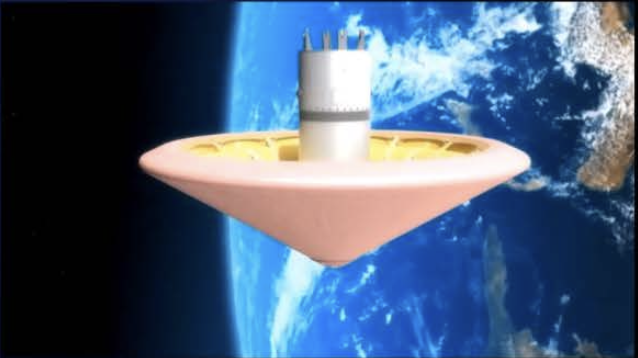
\includegraphics[width=0.5\textwidth]{figures/HIADsDeployed.png}
    \caption{HIADs when deployed}
    \label{fig:Hiaddeployed}
\end{figure}

\par
The development of IADs requires an approach that combines aerodynamics, structural mechanics, and materials science. A key component of an IAD is the flexible thermal protection system (FTPS), which is responsible for protecting the inflatable structure from the intense heat of reentry. The FTPS is a multi-layered system that typically consists of an outer fabric, insulation layers, and a gas barrier~\cite{Guo2011Polyimide}. The design and analysis of the FTPS requires accurate modeling of the aerothermal loads and the material response.

\begin{figure}[H]
    \centering
    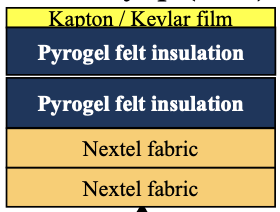
\includegraphics[width=0.5\textwidth]{figures/IADsLayer.png}
    \caption{IADs Layer Example}
    \label{fig:Hiadlayer}
\end{figure}

\section{Problem Statement}
The successful design and operation of an IAD depend on the ability to accurately predict and manage the complex aerothermodynamic environment and the fluid-structure interaction (FSI) phenomena that occur during atmospheric reentry. The flexibility of the IAD structure and the FTPS adds a layer of complexity to the analysis that is not present in traditional rigid heat shields. The deformation of the IAD under aerodynamic loads can affect the flow field and the heat transfer to the vehicle, which in turn can affect the structural response.

At hypersonic speeds ($Ma > 5$) and high altitudes ($> 50$ km), the atmospheric density is sufficiently low that the continuum assumption underlying traditional Computational Fluid Dynamics (CFD) begins to break down. The Knudsen number ($Kn$), which characterizes the degree of rarefaction, increases to values where the Navier--Stokes equations are no longer valid. In this transitional regime, particle-based methods such as Direct Simulation Monte Carlo (DSMC) are required to accurately capture the gas dynamics~\cite{bird1994molecular}.

Furthermore, the optimization of HIAD geometry for survivability -- balancing drag performance, peak heating, ballistic coefficient, and structural mass -- requires an automated, multi-stage computational framework that can efficiently explore a high-dimensional design space. Existing approaches based on parametric CFD sweeps are computationally prohibitive for the thousands of design evaluations required.

Therefore, there is a critical need for an integrated computational framework that: (1) employs DSMC-based rarefied gas dynamics to accurately predict aerothermal loads in the transitional regime, (2) incorporates automated parametric geometry generation for design space exploration, and (3) leverages physics-informed machine learning and surrogate-based optimization to efficiently identify optimal HIAD configurations.

\section{Research Objective}
In this research, the objective is to develop and validate a computational framework for the aerothermal analysis and survivability optimization of a Hypersonic Inflatable Aerodynamic Decelerator (HIAD), based on the SPARTA DSMC solver and integrated with physics-informed neural network (PINN) refinement and genetic algorithm optimization.

The specific objectives are:
\begin{enumerate}
    \item \textbf{Parametric Geometry Generation:} To develop an automated 3D CAD pipeline using CadQuery for generating HIAD profiles based on IRVE-3 specifications, enabling parametric variation of toroid count, cone angle, nose radius, and aeroshell diameter for design space exploration.

    \item \textbf{DSMC Aerothermal Analysis:} To perform high-fidelity rarefied gas dynamics simulations using the SPARTA DSMC solver, capturing the Boltzmann-level molecular collisions and transport phenomena in the transitional flow regime ($0.01 < Kn < 10$) relevant to HIAD reentry at 50--60 km altitude.

    \item \textbf{Knudsen Number Field Mapping:} To analyze the spatial distribution of the Knudsen number across the HIAD surface and surrounding flow field, identifying continuum ($Kn < 0.01$), transitional ($0.01 < Kn < 1$), and free-molecular ($Kn > 1$) regions to characterize the flow physics governing aerothermal loads.

    \item \textbf{Aerothermal Load Prediction:} To determine the surface distributions of heat flux ($\dot{q}$), pressure, and shear stress using the Sutton-Graves stagnation-point correlation and SPARTA surface compute quantities, with validation against IRVE-3 flight data.

    \item \textbf{PINN Flow Field Refinement:} To apply Physics-Informed Neural Networks (DeepXDE) as a post-processing step to smooth noisy DSMC data, fill gaps in the flow field, and provide a continuous interpolant anchored in the compressible Navier--Stokes equations.

    \item \textbf{Survivability Optimization:} To implement a Genetic Algorithm (GA) coupled with a PyTorch-based Metamodel Prognosis (MoP) for automated optimization of HIAD geometry, targeting ballistic coefficient, peak deceleration, backface temperature, and drag performance.
\end{enumerate}

\section{Research Gap}
Based on the literature review, several gaps are identified in the current state of HIAD aerothermal analysis:
\begin{itemize}
    \item \textbf{Rarefied Regime Limitation:} Existing HIAD aerothermal studies predominantly rely on continuum CFD (RANS/LES), which is physically inappropriate for the transitional flow regime ($Kn > 0.01$) encountered at reentry altitudes above 50 km. Particle-based DSMC methods have not been systematically applied to HIAD geometry optimization.

    \item \textbf{Automated Design Space Exploration:} Current approaches require manual parametric sweeps with individual CFD runs, making high-dimensional design optimization (6+ parameters) computationally infeasible. No integrated framework exists that couples automated geometry generation with DSMC simulation and machine learning-based optimization.

    \item \textbf{PINN-DSMC Hybrid Approach:} While Physics-Informed Neural Networks have been applied to CFD post-processing, their use as a smoothing/interpolation layer for noisy DSMC particle data in HIAD applications is unexplored.

    \item \textbf{Multi-Objective Survivability Optimization:} The simultaneous optimization of ballistic coefficient, peak heating, backface temperature, and structural mass for HIAD configurations using surrogate-assisted genetic algorithms has not been demonstrated.
\end{itemize}

\section{Novelty and Contributions}
The present work makes the following novel contributions to the field of hypersonic aerothermodynamic analysis and HIAD design:

\begin{enumerate}
    \item \textbf{First Integrated DSMC-PINN-Optimization Framework for HIAD:} This study presents the first computational framework that couples automated parametric geometry generation (CadQuery), high-fidelity DSMC rarefied gas dynamics (SPARTA), Physics-Informed Neural Network refinement (DeepXDE), and surrogate-assisted genetic algorithm optimization in a unified pipeline for HIAD survivability analysis.

    \item \textbf{DSMC-Based Design Space Exploration:} Unlike prior studies limited to continuum CFD (RANS/LES), this framework employs particle-based DSMC to accurately capture the transitional flow regime ($0.01 < Kn < 10$) encountered at reentry altitudes above 50 km, enabling physically correct aerothermal load prediction for inflatable decelerators.

    \item \textbf{PINN as DSMC Post-Processor:} The application of Physics-Informed Neural Networks as a smoothing and interpolation layer for noisy DSMC particle data is novel in the context of HIAD aerothermal analysis. The two-stage training protocol (data-only followed by data+PDE) provides a physics-consistent continuous field from discrete particle simulations.

    \item \textbf{Multi-Objective Surrogate-Assisted Optimization:} The simultaneous optimization of ballistic coefficient, peak heating, backface temperature, and drag performance using a PyTorch MoP surrogate coupled with a genetic algorithm demonstrates a computationally efficient approach to HIAD design that would be infeasible with direct simulation alone.

    \item \textbf{Comprehensive ML Documentation Standards:} The framework adheres to established machine learning research standards, including explicit architecture documentation, reproducibility requirements (random seeds, environment specifications), validation metrics ($R^2$, RMSE, MAE), and uncertainty quantification through ensemble prediction.
\end{enumerate}

\section{Scope and Limitations}

The scope of this research is defined to provide aerothermal analysis and survivability optimization of the Flexible Thermal Protection System (FTPS) within the constraints of available computational resources. The boundaries and limitations of this study are as follows:

\begin{enumerate}
    \item \textbf{Geometric Representation:} The HIAD structure is modeled using parametric 3D CAD generation via CadQuery (Python scripting). The 6-toroid stack configuration based on the Rapisarda (2023) MDAO baseline is the primary geometry, with the option to vary toroid count, cone angle, and nose radius. The ``scalloped'' toroidal surface is treated as a rigid, fully-inflated geometry to isolate the impact of surface topology on the flow field.

    \item \textbf{Dimensionality:} The investigation supports both 2D axisymmetric (via \texttt{--slice-angle}) and full 3D simulations. The 2D axisymmetric mode assumes zero angle of attack ($\alpha = 0^\circ$) to maintain rotational symmetry, enabling higher particle resolution within computational memory limits. Full 3D simulations are available for off-axis conditions.

    \item \textbf{Numerical Framework:} The gas dynamics are governed by the Boltzmann equation, solved using the Direct Simulation Monte Carlo (DSMC) method as implemented in the SPARTA (Sandia Parallel Algorithm for Real-Time Application) solver~\cite{plimpton2014sparta}. DSMC is valid for rarefied and transitional flows where the continuum assumption fails ($Kn > 0.01$).

    \item \textbf{Gas Model:} A realistic 5-species air model (N$_2$, O$_2$, NO, N, O) with Variable Soft Sphere (VSS) collision physics is employed. This captures the molecular-level interactions including vibrational energy exchange and dissociation reactions relevant to hypersonic entry conditions.

    \item \textbf{Grid and Collision Pairing:} While DSMC is a particle method, a Cartesian computational grid is required to restrict collision pairing to $O(N)$ complexity (within cells) and to provide sampling volumes for macroscopic property accumulation. The grid resolution must be finer than the local mean free path ($\lambda$). A grid-factor of 0.7 (validated against IRVE-3 flight data) is used as the default.

    \item \textbf{Thermal Analysis:} Surface heat flux is estimated using the Sutton-Graves stagnation-point correlation~\cite{sutton1971gravesh}, validated against IRVE-3 flight data. The 1D transient backface temperature model assumes a thermal lag factor ($\eta_{lag} = 0.15$) through the FTPS insulation stack. SPARTA surface kinetic energy quantities are retained as relative shape-ranking signals for the optimizer, not as absolute heat flux values.

    \item \textbf{Optimization:} The Genetic Algorithm explores the design space using Latin Hypercube Sampling (LHS) for initial population generation, with a PyTorch Multi-Layer Perceptron (MoP) as the surrogate model. PINN refinement using DeepXDE is applied during the exploration phase but is bypassed during final validation to eliminate neural network bias.
\end{enumerate}

\section{Methodology Overview}
This study employs a multi-stage computational framework to analyze the aerothermal performance and optimize the survivability of a Hypersonic Inflatable Aerodynamic Decelerator (HIAD). The framework integrates automated parametric geometry generation, DSMC-based rarefied gas dynamics simulation, Physics-Informed Neural Network refinement, and Genetic Algorithm optimization. The methodology is designed to compare a smooth rigid sphere-cone baseline against the scalloped inflatable architecture under identical hypersonic flight conditions. The workflow is illustrated in Figure~\ref{fig:flowchart_ch1}.

\begin{figure}[h]
    \centering
    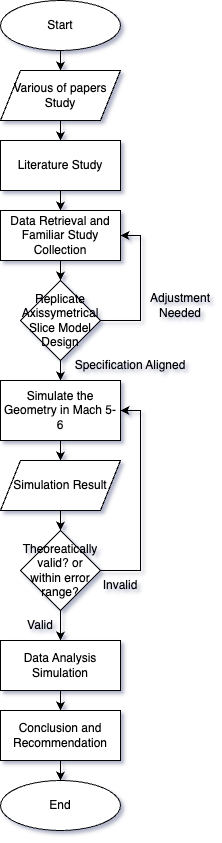
\includegraphics[width=0.85\textwidth]{figures/flowchart.png}
    \caption{Research Methodology Flowchart.}
    \label{fig:flowchart_ch1}
\end{figure}

\subsection*{a. Literature Study}
The initial stage involves a comprehensive literature review of hypersonic aerothermodynamics, rarefied gas dynamics, DSMC methodology, and HIAD design principles. Key topics include the Boltzmann equation, the Direct Simulation Monte Carlo method~\cite{bird1994molecular}, the Sutton-Graves heating correlation, and the IRVE-3/LOFTID flight experiment results. This establishes the theoretical foundation for the computational framework.

\subsection*{b. Parametric Geometry Generation}
The 3D CAD models of the HIAD are generated using CadQuery, a Python-based parametric CAD scripting library. The geometric parameters -- including aeroshell diameter, forebody cone angle, toroid count, toroid radius, and nose radius -- are defined as command-line arguments, enabling automated generation of hundreds of design variants. The output is exported as STL files for SPARTA ingestion.

\subsection*{c. DSMC Simulation}
The SPARTA solver executes the DSMC simulation within a Docker-containerized Linux environment. The simulation domain is initialized with freestream conditions matching the target trajectory point (e.g., $v = 2700$ m/s, $\rho = 6.9674 \times 10^{-4}$ kg/m$^3$ at 52 km altitude from the ISA 1975 model). SPARTA tracks millions of simulated particles, modeling their advection, collisions (VSS model), and surface interactions. Surface computes accumulate force (drag, lift) and energy (heat flux) data, while grid dumps provide field maps of density, temperature, pressure, velocity, and Knudsen number.

\subsection*{d. PINN Refinement}
The raw DSMC output is post-processed using a Physics-Informed Neural Network (PINN) implemented in DeepXDE. The PINN solves the 2D compressible Navier--Stokes equations using automatic differentiation, with SPARTA grid data introduced as observational boundary conditions. The total loss function combines PDE residuals with data-matching terms, providing a smooth, physics-consistent interpolant that fills gaps in the DSMC flow field and reduces particle noise.

\subsection*{e. Survivability Optimization}
A Genetic Algorithm (GA) coupled with a PyTorch Multi-Layer Perceptron (MoP) surrogate model performs multi-objective optimization of the HIAD geometry. Latin Hypercube Sampling (LHS) generates the initial design population. The GA evaluates candidates using the MoP surrogate for rapid screening, with expensive SPARTA simulations reserved for elite candidates and final validation. The cost function balances ballistic coefficient, peak deceleration, backface temperature, and drag performance against user-defined targets.

\subsection*{f. Validation and Analysis}
The simulation results are validated against IRVE-3 flight data~\cite{rapisarda2023mdao} using the Sutton-Graves correlation. Key validation metrics include peak heat flux (14.36\,W/cm$^2$ flight vs.~13.83\,W/cm$^2$ model), total heat load (195.06\,J/cm$^2$ flight vs.~195.17\,J/cm$^2$ model), and peak deceleration (19.7$g$ flight vs.~20.2$g$ model). The final optimized design undergoes a high-fidelity SPARTA validation run \textit{without} PINN refinement to eliminate neural network bias.

\section{Thesis Outline}
The structure of this thesis is arranged as follows. A brief description of each chapter is outlined below:

\textbf{CHAPTER I} This chapter contains the research background, problem statement, research objectives, scope of study, methodology overview, and the systematic thesis outline. This section provides an initial overview regarding the rationale for conducting the research, the specific goals to be achieved, and the limitations of the research scope.

\textbf{CHAPTER II} This chapter contains the theoretical framework and literature review supporting this research. It discusses the fundamental concepts of hypersonic aerothermodynamics, the Boltzmann equation and DSMC methodology, the Sutton-Graves heating correlation, Physics-Informed Neural Networks, and genetic algorithm optimization. This chapter also reviews relevant previous studies including IRVE-3 and LOFTID flight experiments.

\textbf{CHAPTER III} This chapter details the research methodology, covering the automated parametric geometry generation using CadQuery, the SPARTA DSMC simulation configuration, the PINN refinement workflow, the Genetic Algorithm optimization pipeline, and the validation procedures against flight data. It describes the complete computational framework from geometry input to optimized design output.

\textbf{CHAPTER IV} This chapter presents the simulation results and discussion derived from the SPARTA DSMC computational framework. It covers the baseline IRVE-3 geometry configuration, aerothermal surface distributions, flow field characteristics, validation against flight data, and a comparative analysis with prior Newtonian-panel-based approaches highlighting the methodological advances of the present DSMC framework.

\textbf{CHAPTER V} This chapter contains the summary of research findings derived from the data analysis and optimization results. It presents the final conclusions regarding the aerothermal performance and survivability optimization of the scalloped HIAD and provides recommendations for future researchers and aerospace engineers.

\section*{Chapter Summary}
This chapter has established the research context by presenting the background on hypersonic inflatable aerodynamic decelerators (HIADs), identifying the critical need for accurate aerothermal analysis in the transitional flow regime, and defining six specific research objectives. The novelty of this work lies in the first integrated DSMC-PINN-optimization framework for HIAD design, which addresses four identified research gaps in rarefied regime modeling, automated design space exploration, PINN-DSMC hybrid approaches, and multi-objective survivability optimization.

The scope of this research is bounded by the IRVE-3 baseline configuration, 2D axisymmetric and 3D simulations, 5-species air chemistry, and the Sutton-Graves heating correlation. The following chapter presents the theoretical foundations and literature review supporting the computational methodology described herein.
